In this section, we investigate to what extent names annotated in VisualGenome and elicited in ManyNames can be considered canonical, i.e. to what extent speakers agree in their naming choices.
Whereas traditional picture naming studies typically use a prototypical image per category (see Figure~\ref{fig:picture_naming}) and, hence, are mostly interested in the agreement on concept or category-level, we carry out an analysis on two different levels: First, we will look at instances and see to what extent names overlap for the same object. 
Second, we will use the existing annotation of names in VisualGenome to analyze agreement on the level of categories.
\begin{figure}[t]
	\centering
	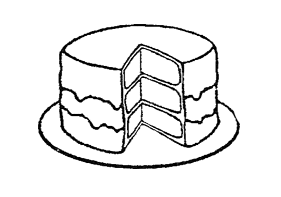
\includegraphics[scale=.5]{figures/snodgrass_vanderwart_cake_042.png}
	\caption{Example of a picture of \textsl{cake} used in traditional picture naming studies (REF to Vanderwart \& Snodgrass) \label{fig:picture_naming}}
\end{figure}


\subsection{Measures}

We compute the following agreement measures:

\begin{itemize}
\item \textbf{\% top}: the average relative frequency of the most frequent response (shown in percent)
\item \textbf{$H$}: the $H$ agreement measure used previously in the psycholinguistic literature
\cs{How is this defined?}
\item \textbf{N}: the average number of types in the response set of ManyNames
\item \textbf{N$_{>1}$}: the average number of types, excluding types that have been annotated only once
\cs{alternatively we could show a plot going from 1 to, let's say, $>10$}
\item \textbf{top=VG}: the proportion of items where the top response in ManyNames corresponds to the VisualGenome name
\item \textbf{\% VG}: the average relative frequency of the VisualGenome name in the response set

\end{itemize}

For measuring \textbf{instance-level agreement}, we consider all names annotated for an object as a response set and then average over these response sets. Furthermore, we compute \textbf{class-level agreement} by merging the response sets for all objects that have the same synset (given for the original VisualGenome name) and compute the measures over these aggregated response sets.
%\gbt{I'd call it ``name-level agreement'' -- it's not really category, is it?}
%\cs{@Sina (referring to our discussion we've had) object class instead of category would imo be indeed clearer here}

\subsection{Results}

Table \ref{tab:agree} shows the analysis of the instance-level and category-level agreement.
On the instance-level, our annotators achieve a fair amount of overlap in their object naming choices. 
Thus, for roughly 70\% of our objects (\textbf{std=?}), the most frequent response in ManyNames corresponds to the original VisualGenome name and, similarly, the average frequency of the top response is also 70\%. 
%Generally, this seems to suggest that indeed many objects in our data set have a canonical name. 
\sz{For NLP people, this looks like a good agreement (given that people were free to type what they wanted). For vision people who might think of it as an object labeling task, this would be pretty low/bad agreement.}
At the same time, the average number of name types per object (5.7, or 2.9 when excluding low-frequency types in each response set) suggests that there is a stable amount of naming variants that is elicited for instances. 
Furthermore, the agreement varies quite considerably among domains \cs{refer to std}:  in the animal domain, which is often discussed in the object naming literature, annotators achieve a very stable and robust agreement of over 90\% and an $H$ agreement which comes close to 0 (where 0 is perfect agreement). 
The people domain, on the other hand, is subject to much more variation and agreement is dramatically lower here, and comes close to 50\% for \% top.



\gbt{Super-interesting results.}
Finally, the category-level agreement figures tell yet another story: when aggregating the responses for all objects with the same VisualGenome synset, we obtain on average 30 types (with $N_{>1})$, i.e. variants of the original VG class. 
Surprisingly, here, only 32.7\% of the aggregated response sets still have the VG name as the most frequent response, which means that for 70\% of the VG names, annotators in ManyNames, on average, prefer a different name.  
Likewise, the relative frequency of the top response drops considerably and $H$ increases from 1.3 for instance-level agreement to 2.4 on object-level agreement.  
\cs{Can we say more about what's going on in the people and vehicles domain, category-level, top=VG? E.g., put corresponding examples in Tab.\ref{tab:qual}}
%
\subsection{Discussion (for now)}
What does this discrepancy between the instance-level and category-level agreement in VisualGenome and ManyNames naming choices mean? 
First of all, it suggests that the same original VisualGenome name can trigger very different variants depending on the visual instance, leading to a drastic increase of variants elicited for categories as compared to instances.
Second, this clearly shows that annotators in VG do not generally annotate the most canonical name \cs{but they don't annotate the name, but the description} and that many names annotated for objects in VG do not correspond to the overall most preferred variant. \sz{think more ...}
\gbt{I don't think we can conclude this second part -- we do have the 70\% top=VG figure that says that VG annotators annotate the most canonical name. What this suggests to me is that instance-level properties are more important than category-level properties, somehow.
  That is, there are systematic properties of instances that make them have a single most salient name.
  However, I expect that this result will be very influenced by referential uncertainty (in single images, it will mostly be clear that it's a man, but in some it may be unclear \ra high instance agreement, low category agrement.}
\cs{I don't think that 70\% is high. E.g., the ResNet has a top-1 error rate of 25\% on ILSVRC 2015.}

\cs{(?!?) With respect to implications for L+V  models on language *interpretation*: much lower agreement on object class-level than on instance-level speaks for using very fine-grained object annotations (as done in ILSVRC). 
	However, that naming variants are often not explained/recoverable by hierarchical relations questions in how far models can understand/interpret reference to objects using more general classes (i.e., names), despite being able to recognise an object's very specific class (e.g., ILSVRC synset). (Relevant?!?)}

\begin{table*}
\footnotesize
\begin{tabular}{p{1.3cm}cccccc|cccccc}
\toprule
 & \multicolumn{6}{c|}{Instance-level agreement} & \multicolumn{6}{c}{Class-level agreement}\\ 
           domain & \% top &    $H$ &    N & N$_{>1}$ & top=VG &  \% VG & \% top &    $H$ &     N & N$_{>1}$ & top=VG &  \% VG \\
\midrule
            all &  69.7 (22.2) &  1.3 &  5.7 &   2.9 &  72.8  &  58.7  &   52.6 (21.1) &  2.4 &   62.2 &  29.7 &  32.7 (46.9) &  23.5 (27.0)  \\
 \midrule
         people &  51.9 (18.1) &  2.1 &  8.6 &   4.3 &         49.8 &         32.3 &     43.1 (14.9) &  2.9 &  104.4 &  53.4 &         24.4 &         13.2  \\
 animals\_plants &  91.3 (12.9) &  0.4 &  2.7 &   1.5 &         93.8 &         88.0 &     67.9 (23.5) &  1.5 &   26.7 &  12.4 &         29.5 &         26.2  \\
       clothing &  63.9 (17.9) &  1.6 &  6.4 &   3.2 &         70.2 &         52.6 &     49.3 (16.6) &  2.6 &   71.7 &  34.1 &         40.5 &         26.1  \\
       vehicles &  72.0 (19.5) &  1.1 &  4.7 &   2.4 &         71.1 &         60.2 &    54.4 (17.4) &  2.1 &   70.4 &  33.2 &         21.4 &         21.3  \\
      buildings &  66.9 (20.5) &  1.5 &  6.9 &   3.0 &         72.6 &         55.5 &      46.7 (18.2) &  3.0 &   68.5 &  31.3 &         32.3 &         22.3  \\
           home &  66.4 (20.5) &  1.5 &  6.3 &   3.1 &         78.5 &         58.8 &     49.6 (18.7) &  2.8 &  103.2 &  48.8 &         45.9 &         30.1  \\
           food &  71.3 (21.1) &  1.3 &  5.5 &   2.9 &         62.9 &         52.1 &     47.3 (19.5) &  2.5 &   32.1 &  15.2 &         31.1 &         20.8  \\
\bottomrule
\end{tabular}\caption{Agreement in naming measured on the level of instances and on the level of VG classes (i.e.\ after grouping objects by their VG synset) \cs{\textbf{std=?})}}
\label{tab:agree}
\end{table*}


%Why is naming more flexible in certain domains than in others? \gbt{Hypothesis: expectation: little variation - hypernymy at most, more variation <-> more affordances <-> more varied relationships.}

\subsection{Qualitative Analysis}

\sz{put qualititative discussion here} Table \ref{tab:qual} shows examples for canonical and non-canonical VG names in our data set, where canonical means that the name was the top response in the aggregated response set in ManyNames.

\begin{table}
\small
\begin{tabular}{lp{4.8cm}r}
\toprule
VG name &  top5 MN names &  n$_{obj}$  \\
\midrule
\multicolumn{3}{c}{\it Canonical VG names with max agreement in MN}\\
 giraffe &  giraffe (96.8), animal (1.2), zebra (0.4), camel (0.3), pole (0.1) &  915 \\
 zebra &  zebra (96.3), animal (1.0), giraffe (0.9), horse (0.2), microwave (0.2) &  461  \\
 cat &  cat (94.8), animal (0.9), kitten (0.8), dog (0.4), laptop (0.2) &  754\\
\midrule
\multicolumn{3}{c}{\it Canonical VG names with min agreement in MN}\\
 booth &  booth (19.3), table (12.3), phone booth (9.8), bench (6.7), building (4.4) &  11 \\
 cabbage &  cabbage (21.4), lettuce (17.0), hotdog (11.9), food (10.7), salad (10.4) &  9 \\
 robe &  robe (22.1), shirt (16.8), jacket (13.3), dress (5.7), clothing (3.2) &  19 \\
  \midrule
  \multicolumn{3}{c}{\it Non-canon. VG names with max agreement in MN}\\
 sedan &  car (88.4), wheel (3.1), vehicle (2.3), automobile (1.3), dog (0.8) &  11 \\
 pony &  horse (83.9), pony (9.1), animal (2.9), donkey (1.1), cow (1.1) &  8 \\
 necktie &  tie (81.4), necktie (10.2), shirt (4.6), ties (1.5), jacket (0.5) &  11 \\
 \midrule
   \multicolumn{3}{c}{\it Non-canon. VG names with min agreement in MN}\\
 shelter &  umbrella (9.7), shelter (8.8), roof (8.0), tent (7.1), building (6.8) &  10 \\
 bath &  shower (13.3), elephant (9.9), birdbath (8.1), water (7.2), trough (7.2) &  10 \\
 vegetable &  food (15.7), broccoli (13.1), sandwich (10.6), salad (9.3), pizza (7.8) &  25 \\
\bottomrule
\end{tabular}
\caption{Examples for VisualGenome (VG) names and their most frequent corresponding responses in ManyNames (MN; percentages shown in brackets). ``Canonical'' means that the VG name is the top name in MN, and non-canonical vice versa.}
\label{tab:qual}
\end{table}

\gbt{The non-canon. VG names suggest that people prefer more general names (``car $>$ sedan'', ``horse $>$ pony'', ``tie $>$ necktie''). Could be due to lexical availability (more general \ra more frequent \ra more available). This could be verified (using frequency). Hypothesis: In cases where top name != VG, the VG name is less general. Could be also a more general hypothesis: see if people prefer more frequent names in general.}
\cs{@Table~\ref{tab:qual} (just wrt presentation) The most interesting blocks are 2 and 3 (canonical VG with min agr.; non-canonical with max agr.)}


\cs{@Table~\ref{tab:agree} I still think that we could also have \%\ top with $N>1$ to give an idea as to how useful the data is for the people interested in using it for, e.g., model evaluation. For that, it is clear that crowdsourcing is noisy and before using it some outlier removal needs to be made.}

% \subsection{Entry-level names and preference orders....}

% \sz{an interesting example:} In our data set, there are 24 images where \textit{penguin} has been used, so we know that the object is a \textit{penguin}. For 50\% of these images, annotators still prefer \textit{bird} as the most common name. According to the theory of entry-level categories, this should not happen. People should always prefer \textit{penguin} over \textit{bird}. 

% \sz{how can we analyze this quantitatively?}

% \begin{itemize}
% \item lettuce -- salad
% \item fruit -- food
% \item man -- catcher
% \item bowl --chili
% \item bowl -- diner \gbt{spelling mistake? should be dinner?} 
% \item burger -- meat
% \item statue -- animal (image shows statue of an animal)
% \item bottle -- alcohol
% \item donut --desert \gbt{spelling mistake? should be dessert?} 
% \item zebra -- stripes
% \item oven -- grill
% \end{itemize}


%%% Local Variables:
%%% mode: latex
%%% TeX-master: "main"
%%% End:
